\documentclass[../main.tex]{subfiles}

\begin{document}
\subsection{Goal}
Our project has two core goals. The first is to develop a model or a collection of models that will build on existing research in
the fields of affective computing, facial expression recognition, and keyboard and mouse dynamics, implementing ideas across these
three fields into a unified model for emotion recognition.

The second goal is to create a software platform that will ease the creation of personalized machine learning software.
The platform will be as implementation-independent as possible to allow the easy integration of research in this field.
The platform will provide utilities that will be necessary for any method trying to create personalized models,
such as data gathering and labeling.


\subsection{Schedule}

\begin{itemize}
    \item \emph{10.12.20 - 12.1.21} - Until the end of the first semester, our goal is to have a working data gathering system.
        Once we can gather the data, our experiments for keyboard and mouse models can start. Until then,
        we will also work on experiments with facial expression recognition that does not require additional data. 
    \item \emph{12.1.20 - 26.2.20} - We expect to focus on gathering additional data during our winter break,
        though we will keep working on experiments that are possible without additional data and start with experiments that require
        little data.
    \item \emph{26.2.21 - 16.4.21} - During the first half of the second semester, we hope to finish most if not all of our experiments,
        possibly adding some more improvements to the data gathering system and maybe even gather some more data. 
    \item \emph{16.4.21 - 18.6.21} - Until the end of the year, we hope to wrap up any remaining experiments, write all the necessary reports,
        and maybe even a paper.
\end{itemize}

\subsection{System Architecture}
In this section, we will give an architecture overview of how the data gathering software should look and operate.
In \ref{fig:system_architecture}, we can see a general architecture. The platform is composed of two major modules:

\begin{figure}[htp]
    \centering
    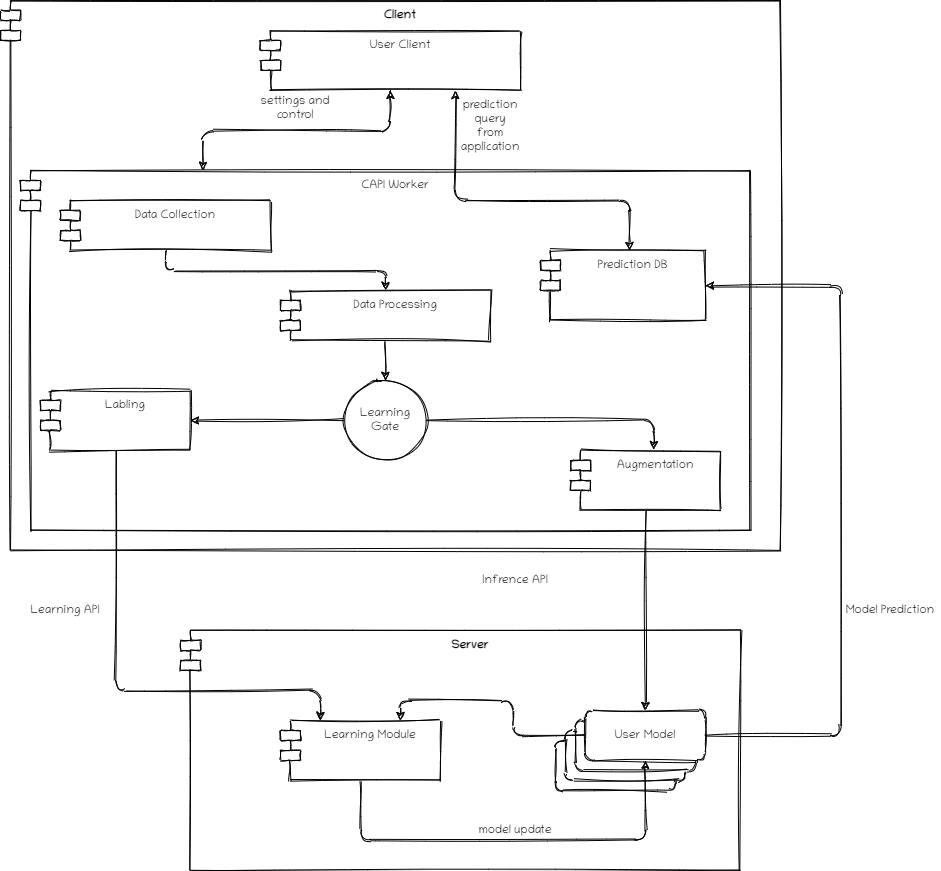
\includegraphics[width=12cm]{figures/platform_architecture.png}   
    \caption{The platform is composed of two major modules. The client runs on the user's computer,
        and is in charge of gathering data whether it is for learning or prediction.
        The server can be in a remote location and is in charge of the harder computations,
        such as training the personal models, and running the models on the user's data.}
    \label{fig:system_architecture} 
\end{figure}

\subsubsection{Client}
The client is also composed of two components. The first is the user client, which is the actual application the user can interact with.
This can come in different forms, but most likely a GUI that will summarize the worker's operations and control its settings,
in addition to using the predictions coming from the server in some way. The second component is the worker. This will most likely be a
separate process running on the user's computer, though it could also run on a different machine depending on the circumstances.
The worker is the mediator between the server, the user client, and the user himself (his data).

\begin{itemize}
    \item \emph{Data Collection} - The data collection module is straightforward. It collects the user's data that is needed for the model to make
        its predictions. This module needs to be very extensible, as different methods might require different data sources and variants.
    \item \emph{Learning Gate} - The learning gate is a simple construct tuned for each model or user. It simply decides when the model needs
        to continue its training. If it decides the model can make a prediction, the data from the Data Collector is passed to the
        Augmentation module. Otherwise, the data will be passed to the learning module.
    \item \emph{Labeling Module} - When the labeling module receives data, it will try to label it (usually by prompting the user).
        Once the data is labeled, it can be sent to the server to train the model. Again the module will be extensible,
        allowing different labeling options to be implemented.
    \item \emph{Augmentation Module} - When data reaches the augmentation module, it means that it needs to get to the server to make a prediction,
        the augmentation module has two goals:
        \begin{enumerate}[i]
            \item \emph{Preprocessing} - usually, a model needs the data to be preprocessed in some way before it can be used,
                as this is a relatively cheap operation, it is performed in the client to save compute time on the server.
            \item \emph{Reduction} - Some models can split in a way that allows one part to reduce the dimensionality of the data and the other to
                make a prediction using the data embedded in the reduced dimension. An excellent example of that is a CNN architecture with
                multiple pooling layers. Because the data is often not small, especially with images or videos, we prefer to run as
                much of the model as possible on the client. If we continue with the CNN example, the image will run through the model's
                first few layers. This will reduce the data's size. The data will be sent over the wire to the server,
                where the rest of the computation will complete. This separation might not always be possible, but when it is, it has the potential
                to save a lot of the time spent transferring the data over the wire.
        \end{enumerate}
    \item \emph{Prediction Database} - The prediction database contains the results of the prediction from the server.
        This is necessary because we might not want to use the results immediately, instead wait for when some event occurs
        (for example, when a news report comes in, the user client will query the
        database and check the user's current mood).
\end{itemize}

\subsubsection{Server}

The server is meant to perform the more expensive computations and will likely not be running on the client machine.
Though we do not disregard the possibility of the server running on the same machine as the client,
a perfect example is if we do not want any of the client's data moving through the internet. The server exposes two APIs:

\begin{itemize}
    \item \emph{Learning API} - the learning API receives requests from the client with labeled data.
        The data from the client is collected and then applied to the client's model during training runs.
    \item \emph{Inference API} - the inference API receives requests from the client with unlabeled data. After it passed through the augmentation module,
        the server runs the client's model on the data and returns the predictions to the client.
\end{itemize}

This paradigm, where each client has a personalized model on the server, can quickly get very expensive.
A few possible improvements can be running part of the model in the augmentation module on the client as discussed before,
Having parts of the model shared between clients. If we use the CNN example again, many of the features will be shared by all clients,
Furthermore, each client will have some additional features and maybe also individual FC layers.
If an ensemble method is used, some models may be shared between multiple or all clients.

\subsection{Experiments}
We can divide our experiments across three categories, facial expression recognition,
keyboard and mouse dynamics, and ensemble. We will also discuss our data gathering techniques here.
\par

We have two types of data gathering. Mood induced data gathering will be performed in a controlled environment. Each participant
will be exposed to a series of videos, movies, games, or some other emotion-inducing media depending on the participant's preferences.
The method of mood induction could be different between participants.
While watching the videos, we will record the participants and label their emotions on the VAD scale and the corresponding
categorical emotions scale. During breaks in the experiment, we will ask the participants to perform some computer tasks and record
their keyboard and mouse. The participants will be recorded during the task, as well. We hope to have at least 10 participants, each recorded
between 1 and 3 hours in this experiment.

A second way we will collect data is using an "out in the wild" experiment. We will let a few people (including ourselves)
install the data gathering system we built and use it for between 1 and 3 weeks. The participants will be occasionally prompted
to label their emotions on the VAD scale. We will collect clips of the participants a few seconds before they are prompted to
label their emotions, as well as the last few seconds, or minutes of keyboard and mouse usage,
and some general statistics of keyboard and mouse use in accordance to what was described in \ref{section:keyboard_mouse}.
\par

For the keyboard and mouse, we have three dimensions along which we need to experiment: model type, personal vs. general model,
classification vs. regression model. We will only use the data we collected for this experiment because we have not found any publicly
available data for keyboard and mouse dynamics with emotion labels. 
\par

The facial expression recognition experiments will be more structured as the model search space is practically infinite.
We will experiment with the three model types we discussed in \ref{section:fer}. Also, experimenting with regression variations of said
models and with personalized variations. We will first focus on the regression vs. classification and model architecture, as most data sets
do not differentiate the participants. Once our data gathering is complete, we will experiment more with making the models personalized.
\par

The ensemble experiments will have to come last in our timeline. Here we will experiment with combining the facial expression models and the
keyboard and mouse models. We will only select some of the best models from each category and use different ensemble methods to combine them.
\par

The most significant uncertainty in our research comes from the data gathering process. Collecting labels that are representative of emotions
is extremely difficult, if not impossible. We hope that our personalized models, regression models, and time series analysis can better use this
labeling than previous methods. Our biggest challenge will be selecting meaningful features, whether it is by modifying our neural network models
or analyzing the keyboard and mouse features.

\subsection{Team Structure}
We have 4 members in our team:
\begin{itemize}
    \item Shoham Zarfati - Works on the facial expression recognition.
    \item Ron Zeidman - Works on the facial expression recognition.
    \item Yuval Khoramian - Works on keyboard and mouse models and physiological aspects of the project.
    \item Hod Twito - Works on keyboard and mouse models and physiological aspects of the project.
\end{itemize}

\end{document}

